\subsubsection{Environment}

\begin{figure}[H]
\centering
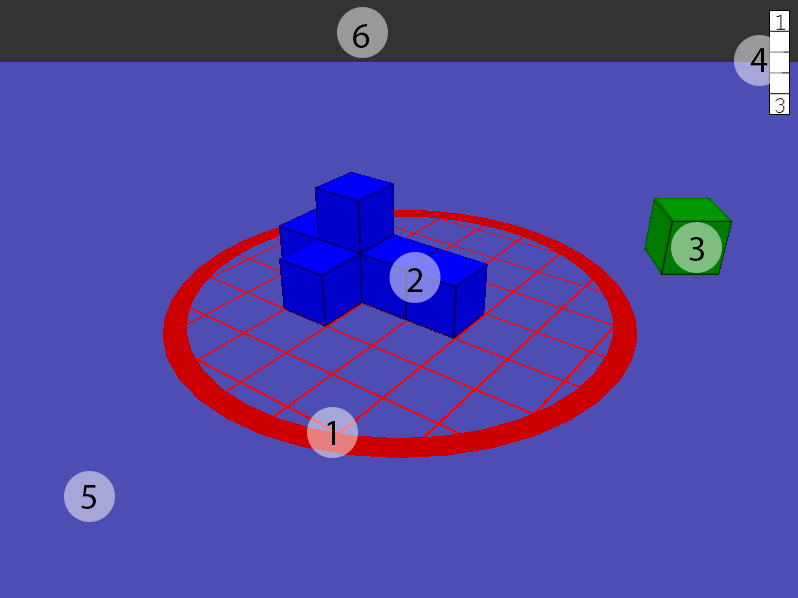
\includegraphics[width=\textwidth]{env_comps}
\caption{\label{fig:environmentcomps} Common rendering of the task environment. Visual elements: 1-Circular~grid 2-Building~blocks 3-Creation~block 4-Target~indicator 5-Floor 6-Horizon}
\end{figure}

\noindent The task environment is a virtual graphical computer program for building virtual block structures using either a LEAP Motion or keyboard and mouse. The environment was developed with the use of jMonkeyEngine~\cite{Irene:2012}, an open source 3D game engine written in Java. For development we used the Software Development Kit that comes with the engine, which provides a high level interface for numerous 3D functions and data-structures (e.g. spatial manipulation, quaternions and 3D meshes) and also provides a high degree of control for developers by being completely compatible with the Java programming language. The environment has been developed for being a general interface were the components could be controlled either through the LEAP Motion or with the keyboard and mouse depending on a simple setting in a configuration file. Therefore most of the components of the environment are utilized by both control strategies. To manipulate the environment with the LEAP Motion device controllers have been developed that employ the LEAP Motion SDK.

Figure~\ref{fig:environmentcomps} shows a common rendering from the task environment in which all visual elements have been labeled. In the center of the screen users are presented with a circular grid that is segmented into several squares, effectively representing a grid with an circular border. On this grid building blocks can be positioned, either directly on the grid or stacked on top of other building blocks. New building blocks can be obtained by interacting (clicking with the mouse or grabbing with the Leap Motion) with the creation block just next to the circular grid. The target indicator on the top right corner gives the user a representation of the block structure that should be created on the grid before the user can move further.

\paragraph{Circular grid}
The circular grid is made out of square grid-cells and a limit circle which has a radius that is slightly bigger than $3.5$ grid-cells width. The grid is able to rotate $360^{\circ}$ around the y-axis of the center of this grid (the origin). In resting state the grid and limit circle have a red color, but while the circle is rotated by the user the limit circle temporarily becomes orange until it reaches resting state once more. 

\paragraph{Building blocks}
The building blocks are 3D cubes with dimensions corresponding to $1\times 1\times 1$ the width of a grid-cell within the grid and all have black outline at the edges. Building blocks can be lifted, dragged around, and dropped by the user. While building blocks are lifted they cast a shadow directly below them in order to know their position relative to the floor and other building blocks. When building blocks are lifted and are within the radius of the grid, they automatically align towards the grid-cells. In resting state the building blocks are blue, when they are being dragged they are orange and when a user points at them, but is not dragging any block, they become light-blue. When building blocks are released they are subjected to gravity, i.e. they fall until they hit the floor or another building block. If building blocks are released outside the circular grid they dissolve and are discarded.

\paragraph{Creation block}
The creation block is an unique building block with the same dimensions as a building block, but with a different color. A user can use the creation block to obtain new building blocks by interacting with it. When a user points at the creation block it turns light-green, otherwise it has a dark-green color. In the version of the environment used for the experiment the creation block was positioned one grid-cell width above the floor level to compensate for the limited vertical detection range of the LEAP Motion. Also depending on the handiness of the user the creation block was either positioned on the left (for left-handed users) or positioned on the right (for right-handed users) of the circular grid.

\paragraph{Target indicator}
The target indicator is a 2D image always visible to the user on the top right of the screen. It shows the currently active target goal structure that must be created by the user with the building blocks in order to advance to the next task and to complete the experiment. The squares corresponds to grid-cells and numbers state the exact amount of building blocks that should be stacked on them. Empty squares should contain no building blocks. The overall image thus depicts the target configuration of building blocks shown in a single orientation, but actual task completion can be achieved by creating a $90^{\circ}$, $180^{\circ}$ or $270^{\circ}$ degree rotated version of the target structure within the grid as well. Also it does not matter where in the grid the solution is created, e.g. a solution structure could be created either in the center or be translated one column to the right: both solutions would suffice. It should be noted however that for task completion the amount of building blocks required for a solution must equal exactly the sum of all the numbers in the target model, i.e. if a solution is created with an additional building block outside the solution then the additional building block should be removed before advancing. See Appendix~\ref{app:models} for the set of target models we used for the experiment.


\begin{figure}[H]
\centering
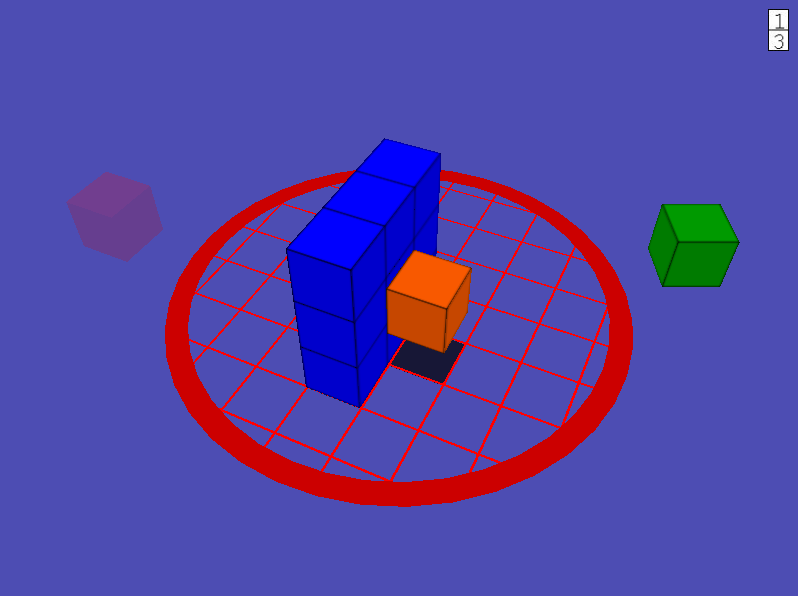
\includegraphics[width=0.47\textwidth ]{ghost_block}
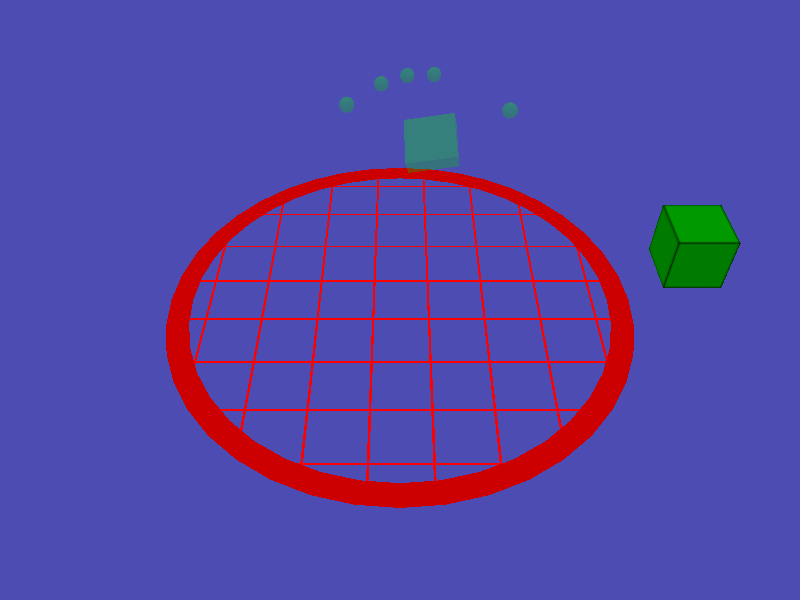
\includegraphics[width=0.47\textwidth ]{leap_hand}
\caption{\label{fig:ghostblock} \textit{On the left:} The ghost block (transparent-red block on the left) appears when a block gets stuck behind other blocks while dragging. In this case the user is dragging a building block from right to left, but the dragged block got stuck behind a wall of other building blocks. \textit{On the right:} The LEAP Motion hand (transparent-green box for the palm, spheres for the finger-tops) is a visualization for when the LEAP Motion device is able to detect one or more hands and the associated fingertips of a user. Additionally it indicates the relative position of the hand palm and fingertips relative to the task environment coordinates. 
}
\end{figure}

\paragraph{Ghost block}
The ghost block is a special transparent-red block that has the same size as a normal building block. It only appears when a building block is dragged but gets stuck behind other blocks. Such a situation is depicted in Figure~\ref{fig:ghostblock} on the left. The ghost block helps the user to realize that an illegal dragging operation is being performed and what the current 3D location of the dragged building block would be if it would not have been stuck.


\paragraph{LEAP Motion hand}
The LEAP Motion hand visualizes the hand of the user when detected by the LEAP Motion device and can be seen in Figure~\ref{fig:ghostblock} on the right. The LEAP Motion hand is only visible to users interacting with the LEAP Motion enabled and helps to relate the relative position of the hands detected by the LEAP Motion device to the coordinates of the task environment. Detected hand palms are represented as flat transparent-green boxes, where the position and orientation are determined by the position and orientation of the users hand palm relative to the LEAP Motion device. Fingertips are represented with small transparent-green spheres and have a position relative to the user fingertips. Each individual fingertip and each hand palm is only shown when it is visible to the LEAP Motion device and hidden otherwise.

\paragraph{Floor}
The floor is merely a purple-blue plane that indicates the lower limit to put the building blocks. It also serves as a surface to project shadows from the building blocks on.

\paragraph{Horizon}
A small strip of horizon is made visible to help the user understand the orientation when tilting the camera up and down. The current color of the horizon is dark-gray.


\paragraph{Color and lighting settings}

All the previously described components have one or more color states associated with them, depending on the state of the respective component and are listed in Table~\ref{tab:colors}. Each  color state consist out of a red (r), green (g), blue (b) and an alpha (a) component contributing to the color intensity and can optionally have a thin black border (outline) at the edges of the objects. Also all visual components, except the horizon, are influenced by two types of virtual lighting: 
\begin{enumerate}
	\item{\textbf{Ambient lighting:}} All color intensities are multiplied by $0.8$ on default.
	\item{\textbf{Parallel directional light:}} All the color intensities of non-transparent object surfaces perpendicular to the y-axis are restored to their original color values.
\end{enumerate}


\begin{table}[H]
\centering
\begin{tabular}{|c|c|c|c|c|c|c|c|}
\hline
\textbf{object} & \textbf{state} & \textbf{r} & \textbf{g} & \textbf{b} & \textbf{a} & \textbf{outline} & \textbf{common name}\\ \hline\hline
Building block & resting & 0 & 0 & 255 & 255 & x & blue \\ 
 & dragged & 255 & 191 & 0 & 255 & x & orange \\ 
 & pointed & 138 & 149 & 255 & 255 & x & light-blue \\ \hline 
Creation block & resting & 0 & 178 & 0 & 255 & x & dark-green \\ 
 & pointed & 158 & 255 & 149 & 255 & x & light-green\\ \hline 
Ghost block & - & 255 & 0 & 0 & 51 & & transparent-red \\ \hline
LEAP Motion hand & - & 0 & 255 & 0 & 77 & & transparent-green  \\ \hline 
Grid & resting & 255 & 0 & 0 & 255 & & red \\ 
 & rotating & 255 & 191 & 0 & 255 & & orange \\ \hline 
Floor & - & 77 & 77 & 179 & 255 & & purple/blue \\ \hline 
Horizon & - & 51 & 51 & 51 & 255 & & dark-gray \\ \hline 
\end{tabular}
\caption{\label{tab:colors} Color states of the objects within the task environment.}
\end{table}

\noindent The rationale for the colors is that a user should be able to clearly differentiate the different components and their states within the environment. The outline of the blocks was added to clearly distinguish between building blocks while they are immediately next to each other. Also, pilot tests without the `pointed' states for the creation block and the building blocks showed that some users struggled to see when they were at the right position with the LEAP Motion hand to properly select and pickup blocks, thus the `pointed' states were included to make this more evident. 

